\documentclass[a4paper,12pt]{article}
\usepackage[utf8x]{inputenc}
\usepackage[T1]{fontenc}
\usepackage[french]{babel}
\usepackage{graphicx}
\graphicspath{ {images/} }
\usepackage{float}
\usepackage{listings}

\setlength{\parindent}{0cm}
\setlength{\parskip}{1ex plus 0.5ex minus 0.2ex}

\title{Organisation de travail}
\author{Mohammad Nauval}

\begin{document}
\maketitle

Dans cette partie, nous allons examiner l'organisation de notre projet. Comme la taille du projet est assez grande et il y a six personnes dans notre équipe, le projet est découpé en plusieurs modules. Les modules sont :

\begin{enumerate}
	\item Analyseur
	\item Compilateur
	\item Interpréteur Minijaja
	\item Interpréteur Jajacode
	\item L'état mémoire
	\item Contrôle de type
	\item Interface homme-machine
\end{enumerate}

Nous avons implémenté l'approche d'agilité dans la réalisation de notre projet. Nous organisons le développement en cycles de quelques semaines. 

Nous avons eu 12 semaines pour finir le projet. Au début du développement, nous avons planifié deux \textit{releases} pour livrer le projet. C'est-à-dire que nous avons eu 6 semaines avant chaque \textit{release}.  

Pour \textit{release} 1, nous avons décidé de réaliser toutes les fonctionnalités du projet. Cependant, celle-ci n'étais logiquement pas possible. En effet, le projet livré pour \textit{relase1} ne fonctionne pas pour la totalité de grammaire Minijaja, il fonctionne pour une grammaire réduite. Le projet était élargi pour couvrir la grammaire complète.

Avant le développement, nous avons défini des fonctionnalités que notre projet doit accomplir. Les fonctionnalités sont ensuite découpées pour chaque \textit{release}. En effet, nous avons les fonctionnalités à accomplir pour \textit{release} 1 ainsi pour \textit{release} 2. Ces fonctionnalités sont définies dans le \textit{backlog} du produit.

\begin{figure}[H]
\begin{center}
	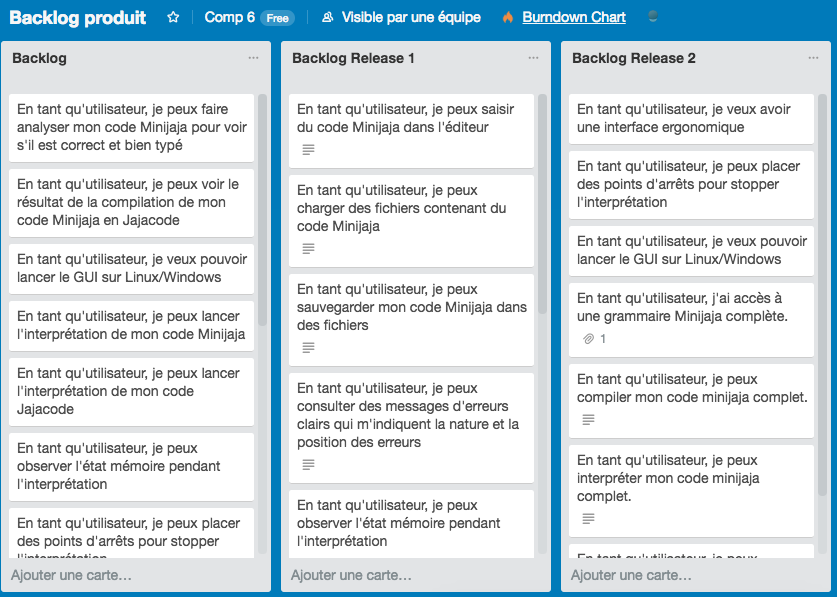
\includegraphics[scale=0.3]{backlogproduit}
	\caption{Backlog produit du projet}
\end{center}
\end{figure}

Comme ce que nous avons déjà mentionné, nous avons 6 semaines avant chaque \textit{release}.

\end{document}